\documentclass[border=8pt]{standalone}
\usepackage{tikz}
\usetikzlibrary{arrows.meta,positioning,calc,decorations.pathmorphing}
\begin{document}
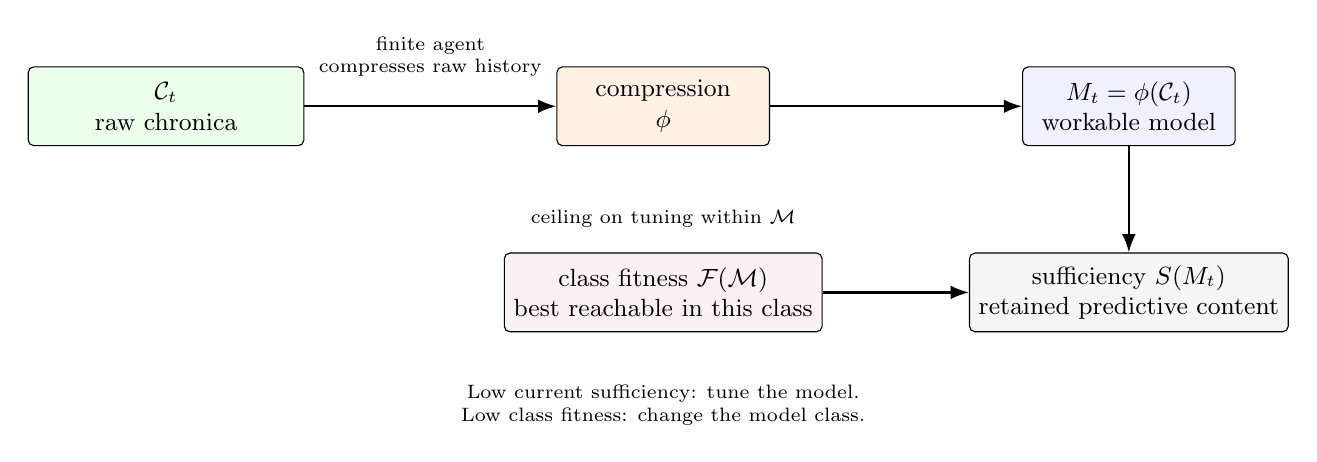
\begin{tikzpicture}[
  box/.style={draw, rounded corners=2pt, align=center, minimum width=2.7cm, minimum height=1.0cm, font=\small},
  arr/.style={-Latex, thick},
  note/.style={align=center, font=\scriptsize}
]

\node[box, fill=green!8, minimum width=3.5cm] (C) {$\mathcal C_t$\\raw chronica};
\node[box, fill=orange!10, right=3.2cm of C] (phi) {compression\\$\phi$};
\node[box, fill=blue!6, right=3.2cm of phi] (M) {$M_t=\phi(\mathcal C_t)$\\workable model};

\draw[arr] (C) -- node[above=0.25cm, note] {finite agent\\compresses raw history} (phi);
\draw[arr] (phi) -- (M);

\node[box, fill=gray!8, below=1.35cm of M, minimum width=3.25cm] (S) {sufficiency $S(M_t)$\\retained predictive content};
\draw[arr] (M) -- (S);

\node[box, fill=purple!6, below=1.35cm of phi, minimum width=3.6cm] (F) {class fitness $\mathcal F(\mathcal M)$\\best reachable in this class};
\draw[arr] (F) -- (S);

\node[note, below=0.55cm of F] {Low current sufficiency: tune the model.\\Low class fitness: change the model class.};
\node[note, above=0.2cm of F] {ceiling on tuning within $\mathcal M$};

\end{tikzpicture}
\end{document}
